\documentclass[a4paper]{article}


\usepackage{amsmath} % using math package
\usepackage{amssymb}

\usepackage{xcolor}
\usepackage{graphicx}

%define new command
\newcommand{\pd}{\partial}


\newcommand{\ket}[1]{\big|  #1 \big \rangle }
\newcommand{\bra}[1]{ \big\langle #1 \big | }

\newcommand {\avg}[3] {\langle {#1} |{ #2} |{#3} \rangle}

    \usepackage{url}


\begin{document}
\title{Understanding Quantum Mechanics by Sequential Stern-Gerlach Experiments (Outline)}
\author{Ting Wang}
\date{10 Dec, 2018}
\maketitle

\begin{abstract}
In this essay, we apply the quantum measure theory to interperate
the results of sequential Stern-Gerlach (SG) experients, which deepens
our understanding of the quantum mechanics.
\end{abstract}

\section{Introduction}
The original SG experiment was given by A and B in some years,
which proved the existence of spin.  The experimental setup is as shown in
Fig. 1.  A beam of Sliver are heated in the oven and then pass  through...,
.... Surprisely, the beams in the screen is not continues as predicted by
classical physics, but discritly separated into two branches.  The result
also can be viewd as one of the simplest quantum system, a two level energy system.

J.J. Sakurai extented the original SG experiment to the sequential ones to illustrate the essential
of quantum mechanics. Here we follow the Sakurai's discussion in \cite{sakurai1994modern} to
demostrate and understand the quantum mechanics itself.
\section{Methods}
\subsection{Sequential SG experiments}

\subsection{Quantum measurement theory}
Now let us apply the quantum measurement theory to calculate the outcomes from
the sequential SG experiments.
...



\section{Results}
The calculation is consisted with the results from SG experients. ...

\section {Conclusion}
The result shows that the results of SG can be calculated and predicted in then
framework of quantum mechanics. The quantum mechanics analysis of the SG Experiments
enhances our believe of the theory.




\begin{figure}[htbp!] \label{sunrise}
\centering % put the fig. in the center
    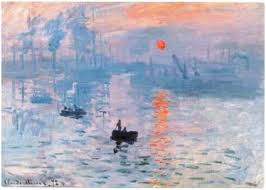
\includegraphics[width=0.8\linewidth]{sunrise.jpg}
    \caption{Sunrise, Claude Monet, 1872}
\end{figure}
\section{Appendix}
\subsection{Details about the original SG experiment}
\subsection{Analogy with light polarization}
\subsection{Hilbert space and Dirac notation}


\bibliographystyle{abbrv}
  \bibliography{Academic_English.bib}

\end{document}
